\documentclass[a4paper,12pt]{article}

\usepackage{graphicx}
\usepackage[margin=2.5cm]{geometry} %%Gestione margini
\usepackage{setspace}  %Gestione interlinea
  \onehalfspacing
\setlength\parindent{1.25cm} %gestione indentazione

\usepackage[parfill]{parskip} %Se necessatrio non indenta, ma inserisce spazio

%Serve per andare a capo nelle colonne
\usepackage{array}
\newcolumntype{L}[1]{>{\raggedright\let\newline\\\arraybackslash\hspace{0pt}}m{#1}}
\newcolumntype{C}[1]{>{\centering\let\newline\\\arraybackslash\hspace{0pt}}m{#1}}
\newcolumntype{R}[1]{>{\raggedleft\let\newline\\\arraybackslash\hspace{0pt}}m{#1}}

%Altro
\usepackage{textcomp}  %%Serve per i gradi Celsius
\usepackage{verbatim}  %%Serve per i commenti lunghi, se ci sono
\usepackage{rotating} %%Seve per mettere le figure in orizzontale
\usepackage[hang,small,bf]{caption} %%Gestisce meglio le didascalie
\newenvironment{smallMargin}[2] %% Serve per ridurre il corpo di fig e tab.
               {\begin{list}{}{\leftmargin#1\rightmargin#2}\item{}}%
               {\end{list}}
\usepackage{hyperref}

%Modifica il font degli headings
\usepackage{sectsty}
\sectionfont{\large\uppercase}
\subsectionfont{\normalsize\bfseries}             
\subsubsectionfont{\normalsize\mdseries\itshape}

%Bibliografia
\usepackage[sort&compress]{natbib}
\bibliographystyle{wre}

%\usepackage[markers, tablesfirst, nolists]{endfloat}  %%figure in fondo

%Gestisce l'elenco figure
\usepackage{tocloft}
\renewcommand*\cftfigpresnum{\textbf{Fig.} ~}
\settowidth{\cftfignumwidth}{\cftfigpresnum}
\renewcommand{\cftfigaftersnumb}{\quad~}
\renewcommand\listfigurename{Figure legends}

%Gestisce la lingua italiana
%\usepackage[utf8x]{inputenc}
%\usepackage[T1]{fontenc}
%\usepackage[italian]{babel}

%Information*******************************************************
\author{}
\date{}
\title{Hydro-time (HT), thermal-time (T) and hydro-thermal-time (HTT) models
for seed germination}

%***************************************************************

%Specific RMarkdown
\usepackage{color}
\usepackage{fancyvrb}
\newcommand{\VerbBar}{|}
\newcommand{\VERB}{\Verb[commandchars=\\\{\}]}
\DefineVerbatimEnvironment{Highlighting}{Verbatim}{commandchars=\\\{\}}
\usepackage{framed}
\definecolor{shadecolor}{RGB}{248,248,248}
\newenvironment{Shaded}{\begin{snugshade}}{\end{snugshade}}
\newcommand{\KeywordTok}[1]{\textcolor[rgb]{0.13,0.29,0.53}{\textbf{{#1}}}}
\newcommand{\DataTypeTok}[1]{\textcolor[rgb]{0.13,0.29,0.53}{{#1}}}
\newcommand{\DecValTok}[1]{\textcolor[rgb]{0.00,0.00,0.81}{{#1}}}
\newcommand{\BaseNTok}[1]{\textcolor[rgb]{0.00,0.00,0.81}{{#1}}}
\newcommand{\FloatTok}[1]{\textcolor[rgb]{0.00,0.00,0.81}{{#1}}}
\newcommand{\CharTok}[1]{\textcolor[rgb]{0.31,0.60,0.02}{{#1}}}
\newcommand{\StringTok}[1]{\textcolor[rgb]{0.31,0.60,0.02}{{#1}}}
\newcommand{\CommentTok}[1]{\textcolor[rgb]{0.56,0.35,0.01}{\textit{{#1}}}}
\newcommand{\OtherTok}[1]{\textcolor[rgb]{0.56,0.35,0.01}{{#1}}}
\newcommand{\AlertTok}[1]{\textcolor[rgb]{0.94,0.16,0.16}{{#1}}}
\newcommand{\FunctionTok}[1]{\textcolor[rgb]{0.00,0.00,0.00}{{#1}}}
\newcommand{\RegionMarkerTok}[1]{{#1}}
\newcommand{\ErrorTok}[1]{\textbf{{#1}}}
\newcommand{\NormalTok}[1]{{#1}}
% Redefine \includegraphics so that, unless explicit options are
% given, the image width will not exceed the width of the page.
% Images get their normal width if they fit onto the page, but
% are scaled down if they would overflow the margins.
\providecommand{\tightlist}{%
	\setlength{\itemsep}{0pt}\setlength{\parskip}{0pt}}

\begin{document}

\maketitle

\tableofcontents
\section{Model development}\label{model-development}

Threshold models have been used to describe seed germination, as
affected by the environmental temperature and water potential. The basic
idea is that seed germination does not take place above/below certain
threshold temperature levels (base temperature: \(T_b\) and cutoff
temperature: \(T_c\), respectively) or below a certain threshold water
potential level (base water potential: \(\Psi_b\)). If these thresholds
are respected, the speed and capability of germination can be described
by using some selected models, characterised by biologically meaningful
parameters.

\emph{{[}NOTE: apart from speed and capability, germination uniformity
has never been considered explicitely, so far{]}.}

These threshold models have been known as hydro-time (HT), thermal-time
(TT) or hydro-thermal-time (HTT) models; they are usually based on the
germination rate (GR), that is the inverse of germination time (t) and
represents the fraction of germination that is accomplished in one day.
In this note, we will:

\begin{enumerate}
\def\labelenumi{\arabic{enumi}.}
\tightlist
\item
  review all the main HT, TT and HTT models that have been used, so far;
\item
  highlight the problems relating to fitting these models
\item
  propose that these models are defined at the individual seed level and
  implemented on the time-to-event platform
\item
  highlight some of the advantages of this platform for HT, TT and HTT
  studies
\end{enumerate}

\subsection{Effect of water potential on GR (HT
models)}\label{effect-of-water-potential-on-gr-ht-models}

According to Bradford (2002), the relationship between GR and water
potential in the substrate is linear, above base water potential level:

\begin{equation}
\left\{ {\begin{array}{*{20}{l}}
    GR = \frac{\Psi - \Psi_b}{\theta_H} \,\,\, if \Psi > \Psi_b\\
    GR = 0 \,\,\, if \Psi < \Psi_b
\end{array}} \right.
\end{equation}

The parameter \(\theta_H\) (hydrotime constant) represents the
germination time for a unit difference between \(\Psi\) and \(\Psi_b\).
It is expressed in MPa \(day^{-1}\) or \(hour^{-1}\) and, while the
expected germination time for a seed changes with \(\Psi\), \(\theta_H\)
remains constant.

In our experience, we have often found that the relationship between GR
and water potential in the substrate may be curvilinear (see figure
below).

\begin{figure}[htbp]
\begin{center}
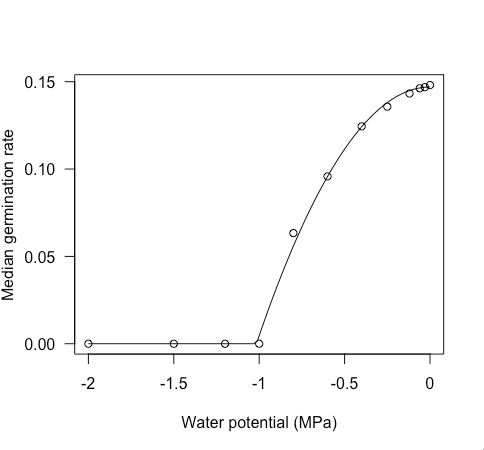
\includegraphics[width=10cm]{_Figures/GRvsPsi_FestAr.png}
\caption{Relationship between germination rate and water potential in \textit{Festuca arundinacea}}
\label{Label}
\end{center}
\end{figure}

For these cases, we have found that the following function may hold:

\begin{equation}
\left\{ {\begin{array}{*{20}{l}}
    GR = \frac{\Psi^2 - \Psi_b^2}{\theta_H} \,\,\, if \Psi > \Psi_b\\
    GR = 0 \,\,\, if \Psi < \Psi_b
\end{array}} \right. \,\,\,\,\,\,\,\,
\end{equation}

In the above equation GR is equal to 0 both with \(\Psi = \Psi_b\) and
\(\Psi = -\Psi_b\); we are obviously interested only in the negative
solution as positive water potential levels are not possible in
practice.

\subsection{Effect of temperature (TT
models)}\label{effect-of-temperature-tt-models}

{[}NOTE: the HT literature generally follows this ordering: HT
-\textgreater{} HTT -\textgreater{} TT models\ldots{} I'll follow a
different line, for now \ldots{}.{]}

According to Garcia-Huidobro et al. (1982), at sub-optimal temperature
levels, the thermal-time (\(\theta_T\), in °C day\(^{-1}\) or
hour\(^{-1}\)) is equal to:

\begin{equation}
\theta_T = (T - T_b) t
\end{equation}

Form the above expression, it follows that:

\begin{equation}
GR = \frac{T - T_b}{\theta_T}
\end{equation}

We see that the germination rate is linearly related to temperature,
with intercept equal to \(-T_b/\theta_T\) and slope equal to
\(1/\theta_T\).

At super-optimal temperature levels a decrease in germination rate is to
be expected, which has been related to a decrease in the ability of
absorbing water from the environment. Several expressions can be found
in literature to describe the above trend

\subsubsection{Broken-stick model, as derived from Alvarado and Bradford
(2002)}\label{broken-stick-model-as-derived-from-alvarado2002_hydrotime}

In this model thermal time stops accumulating at the optimal temperature
level (\(T_o\)) and remains constant. From \(T_o\) onwards, GR decreases
when temperature increases:

\begin{equation}
GR = \left\{ {\begin{array}{*{20}{l}}
0 \rightarrow \,\,\, if \,\,\, T < T_b \,\,\, or \,\,\, T > T_c \\
\frac{T - T_b}{\theta_T} \rightarrow \,\,\, if \,\,\, T_b < T < T_o \\
\frac{T_o - T_b}{\theta_T} \left[ 1 - k (T - T_o) \right] \rightarrow \,\,\, if \,\,\, T_d < T < T_c 
\end{array}} \right.
\end{equation}

The latter expression may be reparameterised to include cutoff
temperature as an explicit parameter:

\begin{equation}
\frac{T_o - T_b}{\theta_T} \left[ 1 - \frac{T - T_o}{T_c - T_0} \right]
\end{equation}

\subsubsection{Model derived from Rowse and Finch-Savage
(2003)}\label{model-derived-from-rowse2003_hydrotime}

The above equation depicts a `broken-stick' trend with a sudden slope
change in \(T_o\), which may not be biologically reasonable. For this
reason, another equation was proposed, where the accumulation of thermal
time occurs for all temperature levels (between \(T_b\) and \(T_c\)),
although such an increase is counteracted by a negative effect starting
from a temperature level equal to \(T_d\), which is close to (but not
coincident with) \(T_o\). The above authors advocated that such a
negative effect is due to an increase in base water potential, that is
shifted upwards at T \textgreater{} \(T_d\), which poses an obstacle to
water absorption.

\begin{equation}
GR = \left\{ {\begin{array}{*{20}{l}}
0 \rightarrow \,\,\, if \,\,\, T < T_b \,\,\, or \,\,\, T > T_c \\
\frac{T - T_b}{\Theta_T} \rightarrow \,\,\, if \,\,\, T_b < T < T_d \\
\frac{T - T_b}{\Theta_T} \left[ 1 - k (T - T_d) \right] \rightarrow \,\,\, if \,\,\, T_d < T < T_c 
\end{array}} \right.
\end{equation}

In the above model, cutoff temperature is obtained when:

\[ k(T - Td) = 1 \]

that is:

\[ T_c = \frac{1}{k} + T_d\]

\subsubsection{Model derived from Mesgaran et al. (2017\ldots{}
hopefully)}\label{model-derived-from-mesgaran-et-al.-2017-hopefully}

According to Mesgaran et al. (2017), the upward shift in base water
potential occurs for all temperatures above \(T_b\). Their equation is:

\begin{equation}
GR = \left\{ {\begin{array}{*{20}{l}}
\frac{T - T_b}{\Theta_T} \left[ 1 - k (T - T_b) \right] \\
GR = 0 \,\,\,\, if \,\,\, T < T_b \,\,\, or \,\,\, T > T_c
\end{array}} \right.
\end{equation}

Here, cutoff temperature is when:

\[ k(T - T_b) = 1\]

that is:

\[ T_c = T_b + \frac{1}{k}\]

\subsubsection{Switch-off functions}\label{switch-off-functions}

In an empirical fashion, we can observe that all the above functions use
a product, wherein the first term represents the accumulation of thermal
time and the second term may be seen as a switch-off term that is 1 when
T = \(T_b\) or T = \(T_d\), decreases when temperature increases and
reaches 0, when T = \(T_c\). Such a decrease represents the effect of
temperature on base water potential and it is linear in all the above
mentioned models.

We could also device other functions where the switch-off is nonlinear.

\subsubsection{Exponential model}\label{exponential-model}

The model below depicts an exponential effect of temperature on base
water potential. The increase in \(\Psi_b\) begins at \(T_b\), it is
small at first and becomes higher as far as the temperature increases.

\begin{equation}
GR = \left\{ {\begin{array}{*{20}{l}}
\frac{T - T_b}{\Theta_T} \left\{ 1 - exp \left[ k (T - T_c) \right] \right\} \\
GR = 0 \,\,\,\, if \,\,\, T < T_b \,\,\, or \,\,\, T > T_c
\end{array}} \right.
\end{equation}

The above equation has been used in Catara et al. (2016) and it is not a
real switch-off function, because the switch off term is 1 when T =
\(-\infty\). Therefore, using the above model, the interpretation of
\(\theta_T\) is slightly different from that of models 5 to 8.
Therefore, we can reparameterise it as:

\begin{equation}
\frac{T - T_b}{\Theta_T} \left\{ \frac{1 - exp \left[ k (T - T_c) \right]}{1 - exp \left[ k (T_b - T_c) \right]}  \right\}  
\end{equation}

\subsubsection{Hyperbolic model}\label{hyperbolic-model}

The following model has been taken from Kropff and Laar (1993) and it
was originally used as a simple yield loss function. It is very
flexible, as it may depict different types of relationships between
temperature and base water potential, according to the value taken by
the parameter q.

\begin{equation}
GR = \left\{ {\begin{array}{*{20}{l}}
\frac{T - T_b}{\Theta_T} \left( 1 - \frac{q \frac{T-T_b}{T_c- T_b} }{1 + (q-1) \frac{T-T_b}{T_c- T_b}}  \right) \\
GR = 0 \,\,\,\, if \,\,\, T < T_b \,\,\, or \,\,\, T > T_c
\end{array}} \right.
\end{equation}

\subsection{Combined effect of temperature and water potential (HTT
models)}\label{combined-effect-of-temperature-and-water-potential-htt-models}

Combine equations above in several forms\ldots{} For example (Mesgaran
et al., 2017):

\[GR = \left\{ {\begin{array}{*{20}{l}}
\frac{(T - T_b) \left[ \Psi - \Psi_b - k (T - T_b) \right]}{\Theta_{HT}}  \\
GR = 0 \,\,\,\, if \,\,\, T < T_b \,\,\, or \,\,\, T > T_c
\end{array}} \right.\]

The hydro-thermal-time (\(\theta_{HT}\)) constant is introduced.

To be expanded\ldots{}

\subsection{Describing a population of
seeds}\label{describing-a-population-of-seeds}

All seed populations are characterised by an apparent variability in
germination time/rate, which is usually measured by way of germination
assays, wherein the number of germinated seeds in Petri dishes (or other
containers) is counted at different times after the beginning of the
experiment. Several authors have hypothesized that the above behaviour
is due to \(\Psi_b\), that is highly variable within the population.
Therefore, HT, TT and HTT models have been so far defined at the
`population' level, i.e.~the seed lot is ideally divided into
sub-populations (germination percentiles: g) and the behaviour of the
sub-population (not the individual behaviour) is described (Bradford,
2002). For instance, equation 1 becomes:

\[\left\{ {\begin{array}{*{20}{l}}
    GR_g = \frac{\Psi - \Psi_b(g)}{\theta_H} \,\,\, if \Psi > \Psi_b(g)\\
    GR_g = 0 \,\,\, if \Psi < \Psi_b(g)
\end{array}} \right. \,\,\,\,\,\,\,\,\]

If we consider e.g.~the 50th percentile \(GR_50\) will be determined by
the median base water potential in the population (\(\Psi_{b(50)}\)),
while 50\% germination will not be achieved if \(\Psi\) is lower than
\(\Psi_b(50)\).

This model is interesting, because it describes germination capacity and
velocity at the same time. However, models cast at the population level
are rather `rigid' and very difficult to fit to data from germination
assays. Indeed the dependent variable for equation above refers to the
whole population of seeds and it is not observable at an individual
level. Therefore, biologists are forced into a `two-steps' fitting
procedure, wherein \(GR_g\) levels are (1) derived from germination
assays, often by using nonlinear regression and, subsequently, (2) used
to parameterise Equation 1 or other similar threshold models, as done
e.g.~in Finch-Savage et al. (1998), Alvarado and Bradford (2002), Rowse
and Finch-Savage (2003), Pace and Benincasa (2010), Hardegree (2006).
This is is suboptimal, at least for two reasons:

\begin{enumerate}
\def\labelenumi{\arabic{enumi}.}
\tightlist
\item
  at the second step, the uncertainty in germination rates observed at
  the first step is neglected (Ritz et al., 2013).
\item
  while it is possible to separately describe the behaviour of the
  subpopulations (GR10, GR30, GR50 and so on), it is not easy to
  describe the population as a whole. For instance, it is immediate to
  depict the time course of germination.
\end{enumerate}

In order to circumvent the above problems, several authors have
re-organised HT or HTT models, based on the time-course for the
proportion of germinated seeds. For example, it is easily shown that,
with simple math and assuming a normal distribution for base water
potential within the population, equation 1 can be re-organised as
follows:

\begin{equation}
G = \phi \left\{ \frac{ [ \psi - \frac{\theta_{H}} {t} - \Psi_{b(50)} ] } {\sigma_{\Psi_b}} \right\}
\end{equation}

where \(G\) is the proportion of germinated seeds at time \(t\) and
\(\phi\) is the cumulative normal distribution. This follows the
original formulation of Bradford (2002), who assumed a normal
distribution for \(\Psi_b\) within the population. Such a hypothesis has
been questioned by several authors who advocated the use of different
(asymmetric) distributions, such as the Weibull (Watt et al., 2010), or
the shifted log-logistic (Mesgaran et al., 2013). This latter equation
is following:

\begin{equation}
G(t,\psi) = \frac{1}{ 1 + \left\{ \frac{ \left[ \psi - \left( \theta_{H}/ t \right) - \Psi_{b(50)} + \mu \right] } {\mu} \right\} ^ \lambda }
\end{equation}

where \(\mu\) and \(\lambda\) are respectively the scale and shape
parameters for the log-logistic distribution.

Independently from the selected distribution, these modified equation
can be directly fit to the results of germination assays, by nonlinear
regression, which avoids the above mentioned two-steps procedure.
However, several other problems arise:

\begin{enumerate}
\def\labelenumi{\arabic{enumi}.}
\tightlist
\item
  nonlinear regression does not account for non-normal, heteroscedastic
  responses (counts), repeated observations on the same experimental
  units over time (lack of independence)
\item
  nonlinear regression cannot account for the uncertainty relating to
  the fact that the exact germination moment is never directly observed,
  as the event takes place between two successive assessment times
  (interval censoring). As the consequence, standard errors for model
  parameters are strongly underestimated (Ritz et al., 2013); even
  though this problem may be minimised by using jackknife/bootstrap
  standard errors (Onofri et al., 2014), we recognise that such computer
  intensive procedures are not generally available in statistical
  packages and they may be rather cumbersome to implement.
\end{enumerate}

Furthermore, both the two-step fitting procedure and nonlinear
regression have the following weaknesses:

\begin{enumerate}
\def\labelenumi{\arabic{enumi}.}
\tightlist
\item
  base water potential is unobservable and immeasurable; it is only
  obtained as the empirical result of a curve fitting process;
\item
  the variability in seed germination time/rate is always rigidly
  determined by the variability in base water potential. Otherwise, we
  argue that, in practice, there is no way to separate the variability
  produced by the stochastic distribution of base water potential from
  that attributable to other potential sources of experimental
  variability (such as seed size, inaccuracies in manipulations,
  environmental variability within the incubator).
\end{enumerate}

\subsection{Model building procedure}\label{model-building-procedure}

In order to build a more general and flexible modelling platform, we
propose that HT, TT and HTT models should be defined at the individual
seed level and not at the sub-population level. Indeed, an alternative
way of expressing the model in Bradford (2002) is:

\begin{equation}
 GR_i = \frac{\Psi - (\Psi_b + \epsilon_i)}{\theta_H}
\end{equation}

where \(\epsilon\) represents the stochastic element describing the
seed-to-seed variability in \(\Psi_b\); sticking to the original
definition, such an element can be assumed as normally distributed
(we'll make it more general later on). If we abandon the assumption that
the stochastic variability of germination times/rates is only due to the
variability in base water potential, we can modify the above equation as
follows:

\begin{equation}
GR_i = \frac{\Psi - \Psi_b}{\theta_H} + \epsilon_i
\end{equation}

For the reasons stated above, we argue that this view is more realistic;
however, it is important to point out that no difference exists between
the two approaches. Indeed, it is easily shown that if base water
potential is the only source of variability and it is normally
distributed with mean equal to \(\psi_{b(50)}\) and standard deviation
equal to \(\sigma_{\psi_b}\), GRs are also normally distributed with
mean \(GR_{50}\) and standard deviation
\(\sigma_{GR} = \sigma_{\psi_b} / \theta_H\).

The advantage of our approach is that the equation 15 represents a
traditional linear model, which can be further generalised to
accommodate other types of error distributions, such as the log-logistic
(Mesgaran et al., 2013):

\begin{equation}
\left\{ {\begin{array}{*{20}{l}}
  GR_{50} = \frac{\Psi - \Psi_b}{\theta_H}\\
  GR_i \sim ll(log(GR_{50}), \sigma)
\end{array}} \right.
\end{equation}

implying that the median GR value in the population (GR50) depends on
water potential, while the individual GRs are distributed according to a
log-logistic PDF (ll), with mean = median = log(GR50) and scale
parameter = \(\sigma\).

The problem with equation 16 is that only a fraction of seeds in a lot
will have \(\Psi < \Psi_b\) and, therefore, they will be able to
germinate in the given environmental conditions. This fraction (Pmax) is
lower than 1 and need to be introduced in equation 16 as a `truncating'
factor:

\begin{equation}
\left\{ {\begin{array}{*{20}{l}}
  Pmax = P(\Psi > \Psi_b) \\
  GR_{50} = \frac{\Psi - \Psi_b}{\theta_H} \,\,\,\, if \Psi > \Psi_b \\
  GR_i \sim ll(log(GR_{50}), \sigma) \cdot Pmax + (1 - Pmax) \\
\end{array}} \right.
\end{equation}

There are three aspects in equation 17 that need to be pointed out:

\begin{enumerate}
\def\labelenumi{\arabic{enumi}.}
\tightlist
\item
  the germination rate \(GR_50\) refers only to the germinated fraction,
  not to the whole seed lot, as in the traditional HT, TT or HTT models.
  Indeed, the above models states that the seed population is a mixture
  of two sub-populations, with proportions Pmax and 1 - Pmax,
  respectively (mixture model);
\item
  the variability of germination rates is not directly related to the
  variability on base water potential. There is an expected \(\Psi_b\)
  value that is estimated for the population, while the variability on
  GR values may be or may not be related to the individual variability
  in this parameter.
\item
  the individual germination rates, as well as the individual
  germination times are not measured with absolute precision, but within
  a range (censored data; see Onofri et al., 2011). For instance, if we
  see that 3 seeds have germinated between day 2 and day 3 (between two
  succeeding monitoring times), we can say that this group of three
  seeds has GR values ranging from a minimum of 1/3 to a maximum of 1/2.
  \emph{{[}NOTE: it would be totally equivalent to say that the
  germination time of this group ranges from 2 to 3{]}}.
\end{enumerate}

For the above aspects, model 17 cannot be fit by traditional nonlinear
regression, but requires maximum likelihood estimation. Ritz et al.
(2013) have shown that a likelihood function can be based on the
standard log-logistic cumulative distribution function (CDF), where GR50
and Pmax are made to depend from water potential and/or temperature.
More generally, we can write:

\[\left\{ {\begin{array}{*{20}{l}}
  Pmax = g(T, \Psi) \\
  GR_{50} = f(T, \Psi) \,\,\,\, if \Psi_b < \Psi \\
  S(GR) = Pmax \cdot \Phi(GR_{50}, \sigma) + (1 - Pmax)\\
\end{array}} \right.\]

where \(\Phi\) is an appropriate CDF (log-logistic, weibull\ldots{}).
S(GR) can be used to build a likelihood function as shown by Ritz et al.
(2013). Indeed, every HT, TT, HTT model can be framed within the
time-to-event platform, commonly known as survival analysis in medical
research, which is the most appropriate modelling platform for seed
germination studies (see for example Hunter et al. (1984), Oí'Neill et
al. (2004), Onofri et al. (2010), Onofri et al. (2011), McNair et al.
(2012), Ritz et al. (2013) and references therein \emph{{[}NOTE: add
MEAD, 2014{]}}).

In particular, every HT, TT or HTT model can be cast as a time-to-event
model by using three `ingredients':

\begin{enumerate}
\def\labelenumi{\arabic{enumi}.}
\tightlist
\item
  one function to describe the relationship between the expected
  proportion of germinated seeds (Pmax) and temperature/water potential.
\item
  for Pmax, one function to describe the relationship between the
  expected germination rate and temperature/water potential;
\item
  a CDF (we used the log-logistic);
\end{enumerate}

It is interesting to note that the time course of germinations can be
easily obtained from the above equation, as:

\begin{equation}
G(t, Temp, \Psi) = \frac{Pmax(T, \Psi)}{1 + exp\left[\frac{log(t_i)-log(1/(GR_{50}(T,\Psi))}{\sigma} \right] }
\end{equation}

\subsection{Advantages of the time-to-event
approach}\label{advantages-of-the-time-to-event-approach}

{[}NOTE: we have already discussed this in our 2011 paper about the
`cure model'. Christian has also discussed this in his 2013 paper{]}.

Adavantages on our side:

\begin{enumerate}
\def\labelenumi{\arabic{enumi}.}
\tightlist
\item
  Flexibility: we can represent every type of relationships between
  germination, temperature and water potential by simply changing how
  Pmax and GR50 are modelled (plug/unplug submodels).
\item
  Correct inferences
\item
  the three main characteristics of seed germination (capability,
  velocity, uniformity) are treated independently (this is also a
  disadvantage, though\ldots{})
\end{enumerate}

Disadvantages

\begin{enumerate}
\def\labelenumi{\arabic{enumi}.}
\tightlist
\item
  Higher level of empiricism
\item
  Less parsimonious (but better fit\ldots{}.)
\end{enumerate}

\subsection{Describing the effect of temperature and water potential on
Pmax}\label{describing-the-effect-of-temperature-and-water-potential-on-pmax}

Unlike the traditional HT, TT and HTT models, every time-to-event model
needs a specific function to model Pmax. Several functions can be used
to this aim.

\subsubsection{Effect of water potential on
Pmax}\label{effect-of-water-potential-on-pmax}

According to the classic hydrotime model, only a fraction of seeds
germinate, corresponding to those seeds with individual base water
potential levels lower than the environmental potential level. Such a
fraction may easily be derived for example from from the Equations 12 or
13, by setting t equal to infinity:

\begin{equation}
G_{max}(\psi) = \phi \left\{ \frac{ [ \psi - \Psi_{b(50)} ] } {\sigma_{\Psi_b}} \right\}
\end{equation}

and:

\begin{equation}
G(t,\psi) = \frac{1}{ 1 + \left\{ \frac{ \left[ \psi  - \Psi_{b(50)} + \mu \right] } {\mu} \right\} ^ \lambda }
\end{equation}

In practice, the maximum proportion of germinated seeds follows a
certain cumulative distribution function (normal, logistic,
log-logistic, extreme value, or other), which is closely related to the
distribution of the individual \(\Psi_{b}\) values within the
population. In our studies, we used a shifted exponential model:

\begin{equation}
\left\{ {\begin{array}{*{20}{l}}
\pi = Germ \times \left[ 1 - exp \left( \frac{ \Psi - \Psi_b }{\sigma} \right) \right] \\
\Psi - \Psi_b = 0 \,\,\,\,\,\,\,\, if \,\,\, \Psi < \Psi_b
\end{array}} \right.
\end{equation}

where (\(1 - Germ\)) will represent a possible fraction of seeds that
will show total inability to germinate, regardless of the environmental
water potential (\textbf{Inability to germinate for reasons that do not
pertain to their inability of absorbing water}). As the base water
potential is highly variable for all seeds in the population, one might
be interested in estimating the =
\(\Psi_{b(50)} = \Psi_{b(50)} - log(0.5) \, \sigma\) ), which might be
included in the model:

\begin{equation}
\left\{ {\begin{array}{*{20}{l}}
\pi = Germ \times \left[ 1 - exp \left( \frac{ \Psi - \Psi_{b(50)} - log(0.5) \, \sigma  }{\sigma} \right) \right] \\
\Psi - \Psi_b = 0 \,\,\,\,\,\,\,\, if \,\,\, \Psi < \Psi_b
\end{array}} \right.
\end{equation}

\subsubsection{Effect of temperature on
Pmax}\label{effect-of-temperature-on-pmax}

According to the traditional TT literature, there is very little
variability in Tb across individuals. Therefore, temperature has a
switch on/off effect on germination, in the sense that all individuals
start germinating all together at Tb. In this case, we can only model
the decrease in germination at superoptimal temperature level, which we
could do by using an exponential equation:

\begin{equation}
Pmax = \left\{ {\begin{array}{*{20}{l}}
Germ \left\{ 1 - exp \left[ -k (T_c - T) \right] \right\}\\
0 \,\,\, if \,\,\, T < t_b
\end{array}} \right.
\end{equation}

Our experience suggest that in some populations there is a marked
variability in \(T_b\) across individuals, so that the relationship
between Pmax and Tb will show an increasing trend just above Tb, a more
or less flat peak and a decrease. In order to model this trend, we used
the following equation:

\begin{equation}
Pmax = \left\{ {\begin{array}{*{20}{l}}
Germ \left\{ 1 - exp \left[ -k_1 (T - T_b) \right] \right\} \left\{ 1 - exp \left[ -k_2 (T_c - T) \right] \right\}\\
0 \,\,\, if \,\,\, T < t_b \,\,\, or \,\,\, T > T_c
\end{array}} \right.
\end{equation}

\subsubsection{Combined effect of temperature and water potential on
Pmax}\label{combined-effect-of-temperature-and-water-potential-on-pmax}

yet to be done \ldots{}.

\subsection*{References}\label{references}
\addcontentsline{toc}{subsection}{References}

\hypertarget{refs}{}
\hypertarget{ref-Alvarado2002_Hydrotime}{}
Alvarado, V., Bradford, K., 2002. A hydrothermal time model explains the
cardinal temperatures for seed germination. Plant, Cell and Environment
25, 1061--1069.

\hypertarget{ref-Bradford2002_HydroTime}{}
Bradford, K., 2002. Applications of hydrothermal time to quantifying and
modeling seed germination and dormancy. Weed Science 50, 248--260.

\hypertarget{ref-catara_threshold_2016}{}
Catara, S., Cristaudo, A., Gualtieri, A., Galesi, R., Impelluso, C.,
Onofri, A., 2016. Threshold temperatures for seed germination in nine
species of Verbascum (Scrophulariaceae). Seed Science Research 26,
30--46.

\hypertarget{ref-Finch-Savage1998_HTTM}{}
Finch-Savage, W.E., Steckel, J.R.A., Phelps, K., 1998. Germination and
post-germination growth to carrot seedling emergence: Predictive
threshold models and sources of variation between sowing occasions. New
Phytologist 139, 505--516.

\hypertarget{ref-GarciaHuidibro1982_HTTM}{}
Garcia-Huidobro, J., Monteith, J., Squire, R., 1982. Time, temperature
and germination of pearl millet (pennisetum typhoides s \& h.). 1.
constant temperatures. Journal of Experimental Botany 33, 288--296.

\hypertarget{ref-Hardegree_2006}{}
Hardegree, S., 2006. Predicting germination response to temperature. 1.
cardinal-temperature models and subpopulation-specific regression.
Annals of Botany 97, 1115--1125.

\hypertarget{ref-Hunter1984_SeedGermMethod}{}
Hunter, E., Glasbey, C., Naylor, R., 1984. The analysis of data from
germination tests. Journal of Agricultural Science 102, 207--213.

\hypertarget{ref-kropff_modelling_1993}{}
Kropff, M.J., Laar, H.H. van, 1993. Modelling crop-weed interactions.
CAB International, Books.

\hypertarget{ref-McNair_2012SurvivalSeed}{}
McNair, J.N., Sunkara, A., Frobish, D., 2012. How to analyse seed
germination data using statistical time-to-event analysis:
Non-parametric and semi-parametric methods. Seed Science Research 22,
77--95.

\hypertarget{ref-Mesgaran2013_SeedGermDistributions}{}
Mesgaran, M.B., Mashhadi, H.R., Alizadeh, H., Hunt, J., Young, K.R.,
Cousens, R.D., 2013. Importance of distribution function selection for
hydrothermal time models of seed germination. Weed Research 53, 89--101.

\hypertarget{ref-ONeill2004_FittingComparingSeedGerminationModels}{}
Oí'Neill, M.E., Thomson, P.C., Jacobs, B.C., Brain, P., Butler, R.C.,
Turner, H., Mitakda, B., 2004. Fitting and comparing seed germination
models with a focus on the inverse normal distribution. Australian and
New Zealand Journal of Statistics 46, 349--366.

\hypertarget{ref-OnofriEtAl2010_Survival}{}
Onofri, A., Gresta, F., Tei, F., 2010. A new method for the analysis of
germination and emergence data of weed species. Weed Research 50,
187--198.

\hypertarget{ref-onofri_experimental_2014}{}
Onofri, A., Mesgaran, M., Neve, P., Cousens, R., 2014. Experimental
design and parameter estimation for threshold models in seed
germination. Weed Research 54, 425--435.

\hypertarget{ref-OnofriEtAl2011_CureModel}{}
Onofri, A., Mesgaran, M.B., Tei, F., Cousens, R.D., 2011. The cure
model: An improved way to describe seed germination? Weed Research 51,
516--524.

\hypertarget{ref-PaceIJA_2010}{}
Pace, R., Benincasa, P., 2010. Effect of salinity and low osmotic
potential on the germination and seedling growth of rapeseed cultivars
with different stress tolerance. Italian Journal of Agronomy 5, 69--77.

\hypertarget{ref-Ritz2012_CureModel}{}
Ritz, C., Pipper, C.B., Streibig, J.C., 2013. Analysis of germination
data from agricultural experiments. European Journal of Agronomy 45,
1--6.

\hypertarget{ref-Rowse2003_Hydrotime}{}
Rowse, H., Finch-Savage, W., 2003. Hydrothermal threshold models can
describe the germination response of carrot (\emph{daucus carota}) and
onion (\emph{allium cepa}) seed populations across both sub- and
supra-optimal temperatures. New Phytologist 158, 101--108.

\hypertarget{ref-Watt2010_Hydrotime}{}
Watt, M.S., Xub, V., Bloombergb, M., 2010. Development of a hydrothermal
time seed germination model which uses the weibull distribution to
describe base water potential. Ecological Modelling 221, 1267--1272.


\end{document}
